\documentclass[pdf]{beamer}
\usepackage[latin1]{inputenc}
\usepackage{multirow}
\usetheme{Berkeley} %Warsaw
\usecolortheme{dove}


\begin{document}

\title[Restriction-site Associated DNA tags (RADseq)]{RADseq}
\subtitle{BCB 504: Applied Bioinformatics\\}
\author[Matt Settles]{Matt Settles}
\institute{University of Idaho\\ Bioinformatics and Computational Biology Program}
\date{\today}


%% Title page
\begin{frame}[plain]
  \titlepage
\end{frame}


%% Outline
\begin{frame}[plain] 
  \frametitle{Outline}
  \tableofcontents
\end{frame}

\section{Introduction}
\begin{frame}
  \frametitle{RAD-seq Introduction}
Restriction-site associated DNA (RAD) markers are a type of genetic marker which can be useful for
\begin{itemize}
\item Association mapping
\item QTL-mapping
\item population genetics (population structure)
\item ecological studies
\item pedigree mapping
\item evolution (phylogeny)
\end{itemize}
RAD-seq is a genomic reduction (reduced representation) technique, where you only sequence regions neighboring a particular restriction site(s) allowing you to (1) reduce costs associated with library preparation and (2) pool many more individuals per sequencing run.
\end{frame}

\begin{frame}
 \frametitle{Restriction fragment}
A restriction fragment is a DNA fragment resulting from the cutting of DNA by a restriction enzyme. Each restriction enzyme is highly specific, recognizing a particular short DNA sequence (restriction site), and cutting both strands at specific points within the site. Most restriction sites are palindomic are are 4 to 8 nucleotides long. The shorter the rescriction site the higher number of probable occurances in the genome.
\begin{center}

\includegraphics[scale=1.0]{Figures/Restriction_enzyme.jpg} 
\end{center}
\end{frame}

\begin{frame}
  \frametitle{RAD-seq Library Prep}
\begin{center}
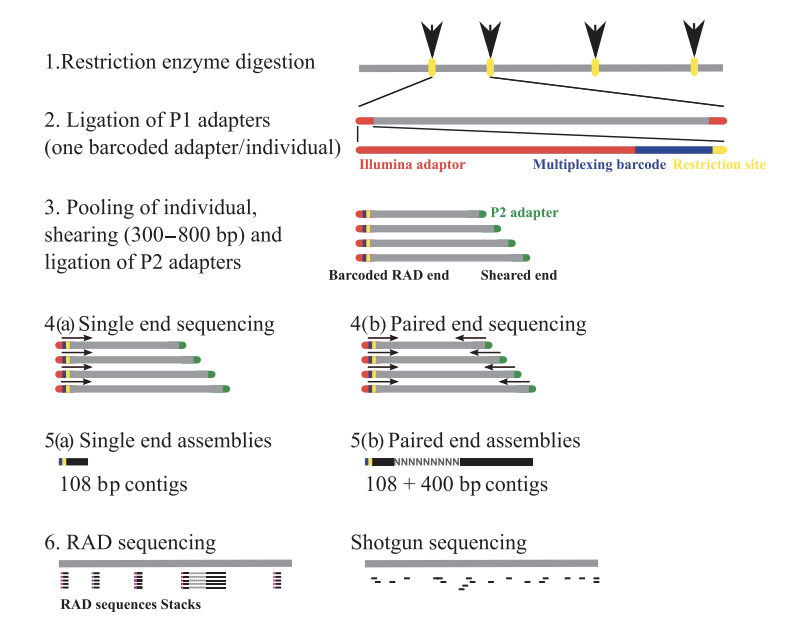
\includegraphics[scale=0.35]{Figures/RADseq.png} 
\end{center}
\end{frame}

\begin{frame}
\frametitle{Double Digest RADseq}
Double Digest RADseq, uses two cutters (one rare and one common) in order to further reduce the number of RAD tags and descrease the cost and complexity of the library preparation. ddRADseq removes the need to randomly shear the DNA and blunt end repair, allowing for initial DNA quantities as low as 100ng. 
\begin{center}
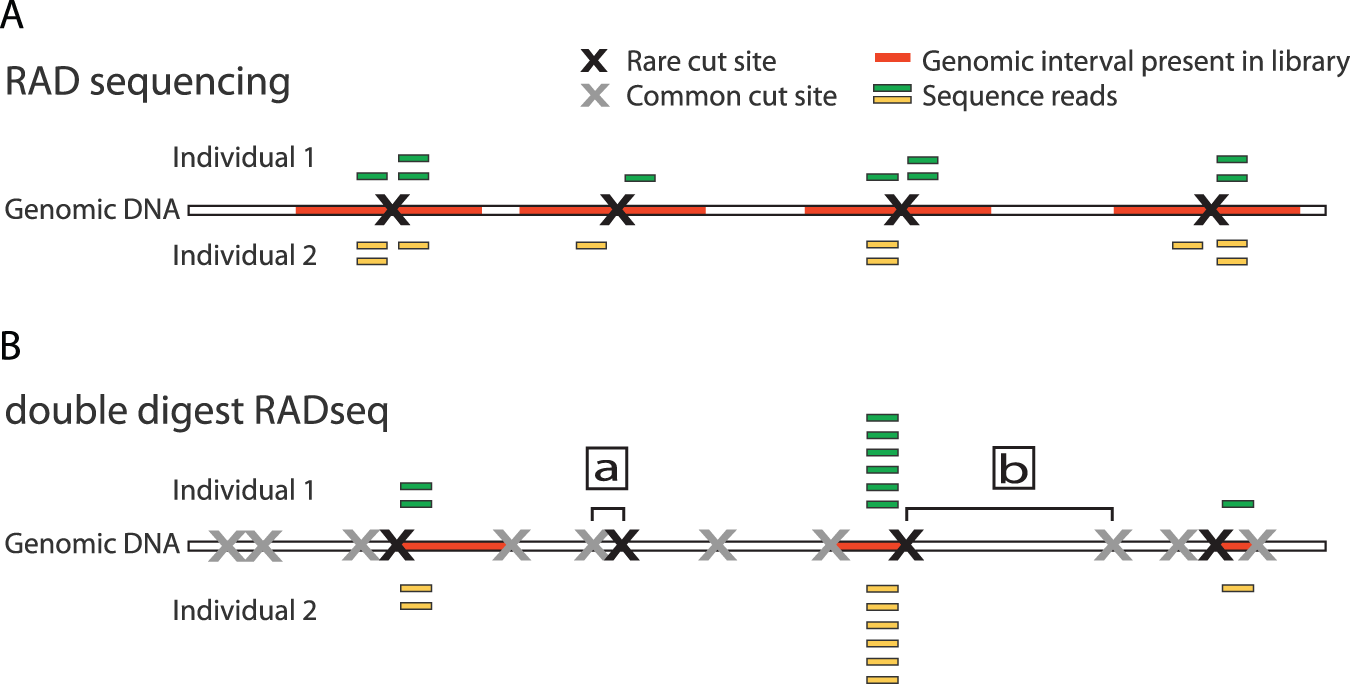
\includegraphics[scale=0.70]{Figures/ddRadseq.png} 
\end{center}
\end{frame}

\begin{frame}
\frametitle{Other similar techniques}
\begin{description}
\item[RRL] Reduced Represetation Library
\item[GBS] Genotype By Sequencing 
\item[CRoPS] Complexity Reduction of Polymorhpic Sequences
\item[MSG] Multiplex Shotgun Genotyping
\end{description}
All techniques rely on restrction enzyme digestion and size selection on a gel
\end{frame}

\begin{frame}
\frametitle{RRL, GBD, RAD technique comparison}
\begin{center}
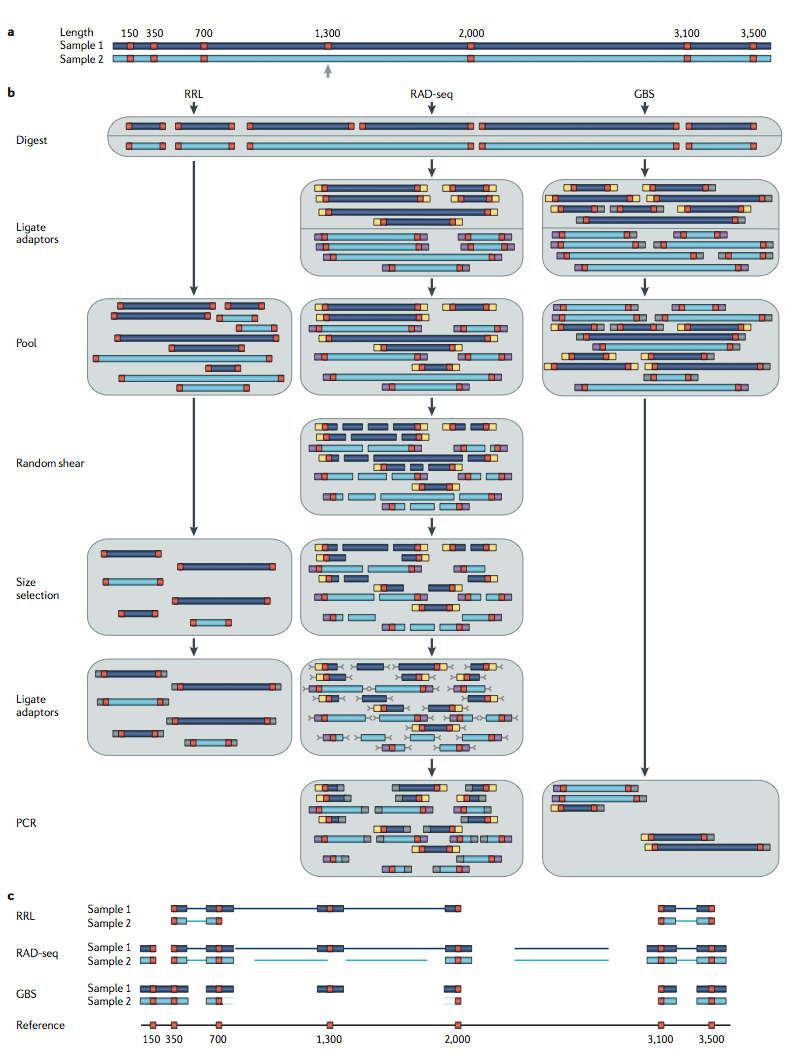
\includegraphics[scale=0.20]{Figures/comparison.png} 
\end{center}
\end{frame}

\begin{frame}
\frametitle{Advantages}
\begin{itemize}
\item Requires no prior knowledge of genome (unlike SNP-chip)
\item Has no ascertainment bias
\item Can pool many, many individuals
\item Tags are homologous across individuals
\end{itemize}
\end{frame}

\begin{frame}
\frametitle{Experimental Design}
Number of sites versus Depth of sequencing per site versus number of samples.
\begin{itemize}
\item Rescriction site and genome size correlate with the number of tags.
\item Depth per tag - target mean depth of 20-40 to call genotypes
\item Use number of sequencing reads and above to determine number of samples that can be pooled.
\end{itemize}
\end{frame}

\begin{frame}
\frametitle{Bioinformatics}
RAD-seq works because you should be sampling the same sites across many individuals. For bioinformatics you need to idendify reads which belong to the same 'tag', determine homologous 'tags' across individuals, pileup tags and call variants. If the genome is known you can additionally align to the genome and add in linkage information.
\end{frame}

\end{document}

